%%%%%%%%%%%%%%%%%%%%%%%%%%%%%%%%%%%%%%%%%%%%%%%%%%%%%%%%%%%%%%%%%%%%%%%%%%%%%%%
%  Key Topics in Artificial Intelligence -- Open Universiteit
%
%  Paper : Evaluating FaceNet resilience under extreme physical and
%          environmental stress: A case study based on Das Boot.
%  Format: ICML 2021 two-column template (camera-ready / "accepted" mode).
%
%  Files in this folder
%    main.tex        -- this file, the paper itself
%    references.bib  -- BibTeX database; every \cite{key} must exist here
%    icml2021.sty    -- ICML 2021 style file  (official ICML template)
%    icml2021.bst    -- ICML 2021 bibliography style (official ICML template)
%    figures/        -- all figures referenced with \includegraphics
%
%  Build (from this folder):
%    latexmk -pdf main.tex        (or: pdflatex, bibtex, pdflatex, pdflatex)
%
%  Status of the sections
%    Abstract ................ TODO
%    Brief Introduction ...... draft
%    Related works ........... draft
%    Methods ................. TODO (still template text + example figures)
%    Experimental Results .... TODO (still template text + example table)
%%%%%%%%%%%%%%%%%%%%%%%%%%%%%%%%%%%%%%%%%%%%%%%%%%%%%%%%%%%%%%%%%%%%%%%%%%%%%%%

\documentclass{article}

% ---------------------------------------------------------------------------
% Packages
% ---------------------------------------------------------------------------
% Recommended, but optional, packages for figures and better typesetting:
\usepackage{microtype}
\usepackage{graphicx}
\usepackage{subfigure}
\usepackage{booktabs} % for professional tables
\usepackage{multirow}
% hyperref makes hyperlinks in the resulting PDF.
% If your build breaks (sometimes temporarily if a hyperlink spans a page)
% please comment out the following usepackage line and replace
% \usepackage{icml2021} with \usepackage[nohyperref]{icml2021} above.
\usepackage{hyperref}

% Attempt to make hyperref and algorithmic work together better:
\newcommand{\theHalgorithm}{\arabic{algorithm}}

% The [accepted] option prints the author names (camera-ready layout).
% Remove it to get the anonymous "under review" layout.
\usepackage[accepted]{icml2021}

% Short title shown in the running header of every page.
\icmltitlerunning{FaceNet Resilience Under Physical and Environmental Stress}

\begin{document}

% ---------------------------------------------------------------------------
% Title block and authors (spans both columns)
% ---------------------------------------------------------------------------
\twocolumn[
\icmltitle{Evaluating FaceNet resilience under extreme physical and environmental stress: A case study based on \textit{Das Boot}.}

\begin{icmlauthorlist}
% TODO: replace "Student Number 1" with the actual student number.
\icmlauthor{Marc S. P. Vlasblom (Student Number 1)}{ou}
\icmlauthor{Patricia de Wit (835622186)}{ou}
\icmlauthor{Duncan R. van der Heul (852908113)}{ou}
\end{icmlauthorlist}

\icmlaffiliation{ou}{Open Universiteit}
\icmlcorrespondingauthor{}{}

% You may provide any keywords that you
% find helpful for describing your paper; these are used to populate
% the "keywords" metadata in the PDF but will not be shown in the document
\icmlkeywords{}

\vskip 0.3in
]

% ---------------------------------------------------------------------------
% Abstract  (TODO)
% ---------------------------------------------------------------------------
\begin{abstract}
    Write a short abstract that contains a brief summary of the work and describes the main points you want to make.

\end{abstract}

% ---------------------------------------------------------------------------
% 1. Introduction: FaceNet, the Das Boot case study, research questions
% ---------------------------------------------------------------------------
\section{Brief Introduction}
Automated face recognition has advanced significantly with deep learning frameworks. A foundational milestone in this domain is FaceNet, introduced by Schroff et al. \cite{schroff2015facenet}. FaceNet maps facial features into a compact, 128-dimensional vector space. By calculating the Euclidean distance between a reference image vector and a test frame vector, the system recognizes individuals. A small distance confirms a match, while a large distance indicates distinct identities. Under controlled or optimal laboratory conditions, this approach achieves exceptionally high accuracy.
\par However, the performance of these algorithms drops significantly under challenging, real-world conditions. To investigate these limitations under extreme circumstances, this study utilizes a unique case study based on the movie Das Boot. This film provides an ideal testing ground because it perfectly replicates severe human fatigue and harsh environmental hardships. Specifically, analyzing this footage introduces three extreme, real-world challenges that commonly disrupt face recognition in practice:
\begin{itemize}
    \item First, the movie features severe technical degradation, containing low-resolution inputs with small, blurry faces far from the camera.
    \item Second, the characters experience extreme physiological changes due to prolonged stress and fatigue, resulting in sweat, dirt, and changing facial hair over time.
    \item Third, the submarine environment suffers from harsh environmental conditions, characterized by deep darkness and low-contrast red alarm lights.
\end{itemize}

Our research question is: How do low resolution, changing faces, and bad lighting in Das Boot influence the performance of the FaceNet recognition algorithm?

our sub questions are:
% Each sub-question maps onto one stress test (1: resolution, 2: appearance,
% 3: lighting) and onto one subsection of the related work below.
\begin{enumerate}
    \item How does low image resolution affect FaceNet's accuracy, and can pixel interpolation effectively mitigate this drop in performance?
    \item To what extent do changing faces due to severe stress and fatigue lower recognition rates, and does adding extra reference photos resolve this issue?
    \item How does poor submarine lighting affect facial feature extraction, and does adding a CLAHE pre-processing step improve the local contrast and model accuracy?
\end{enumerate}

% ---------------------------------------------------------------------------
% 2. Related work: one subsection per stress test
% ---------------------------------------------------------------------------
\section{Related works}

To contextualize how face recognition algorithms perform under extreme conditions, this chapter reviews the existing literature across three key domains: low-resolution imagery, facial appearance changes, and contrast enhancement under poor lighting.

% --- Stress Test 1: low resolution -----------------------------------------
\subsection{Technical Degradation: Low-Resolution Face Recognition}
When face recognition systems shift from controlled environments to real-world applications, technical data degradation becomes a major obstacle. As comprehensively reviewed by Cheng and Zhu \cite{cheng2024}, standard face recognition models inherently fail when processing low-resolution inputs. This failure stems primarily from a critical lack of pixel density.

In low-resolution scenarios, such as when characters are positioned far away from the camera, the structural details of the face are lost. Cheng and Zhu \cite{cheng2024} demonstrate that this missing information severely compromises two crucial pipelines within the recognition process: feature extraction and face alignment. Without precise alignment and distinct feature extraction, the resulting face embeddings become unstable, leading to a sharp increase in error rates.

To bridge this domain gap, recent work by Luévano García et al. \cite{luevano2026} evaluates mitigation strategies under limited data constraints. A prominent trend has been the deployment of heavy generative AI models that attempt to reconstruct high-resolution photos by artificially creating sharp, minute details. However, Luévano García et al. \cite{luevano2026} prove that these heavy generative models often fail to produce a stable and reliable embedding for the actual classification step, as the artificial details frequently distort unique identity traits. Instead, their experimental findings reveal that simpler, geometric adjustments provide significantly more robust performance. Specifically, they demonstrate that combining simple interpolation-based resizing with a diverse database of low-quality reference images yields the highest stability. These insights directly justify our approach for Stress Test 1.

% --- Stress Test 2: changing facial appearance -----------------------------
\subsection{Physiological Degradation: Changing Facial Appearances}
In addition to technical resolution issues, face recognition models must handle severe variations in human appearance over time. This challenge is highly relevant when analyzing characters within a narrative timeline. Research by Abdalah and Alkazaz \cite{abdalah2025} focuses specifically on the complexities of recognizing actors in real movie productions using machine learning.

Using the \textit{Arab Actors Dataset}, Abdalah and Alkazaz \cite{abdalah2025} describe the extreme challenges that elements like makeup, beard growth, wigs, and aging introduce when trying to match faces. Their findings conclude that standard models struggle heavily when a face significantly alters from its original baseline appearance. To overcome this, the study emphasizes that cross-appearance samples---meaning extra reference images that capture the person in various altered states---are strictly needed to maintain recognition accuracy. This conclusion provides the academic foundation for Stress Test 2, where we systematically evaluate the system's performance with and without these extra reference images.

% --- Stress Test 3: poor lighting / contrast -------------------------------
\subsection{Environmental Degradation: Contrast and Bad Lighting}
The final major challenge relates to the operational environment, which frequently suffers from poor illumination. In deep-sea or submarine environments, face recognition is heavily disrupted by extreme darkness and low-contrast color filtering, such as red alarm lighting. Poor lighting hides essential facial gradients, making it nearly impossible for standard models to locate landmarks or map features accurately.

To mitigate this environmental challenge, digital image preprocessing is required before the images are fed into the face recognition algorithm. A widely accepted solution in literature is Contrast Limited Adaptive Histogram Equalization (CLAHE), originally formalized by Zuiderveld \cite{zuiderveld1994}. Unlike standard histogram equalization, CLAHE enhances the local contrast of an image in small, localized patches while preventing the over-amplification of noise in dark areas. This technique brings out hidden facial boundaries and structural details in poorly lit frames, providing the theoretical basis for our approach in Stress Test 3.

% ---------------------------------------------------------------------------
% 3. Methods  (TODO -- template text; the two figures below are placeholders)
% ---------------------------------------------------------------------------
\section{Methods}
Describe the methods used. How it works. It can include algorithms, system descriptions, new language constructs, analyses, etc.
Provide diagrams to help in the discussion. Figure \ref{fig:one-col-figure} and Figure \ref{fig:two-col-figure} shows an example of a one-column figure and a two-column figure.

% One-column figure (width = one column).
\begin{figure}
    \centering
    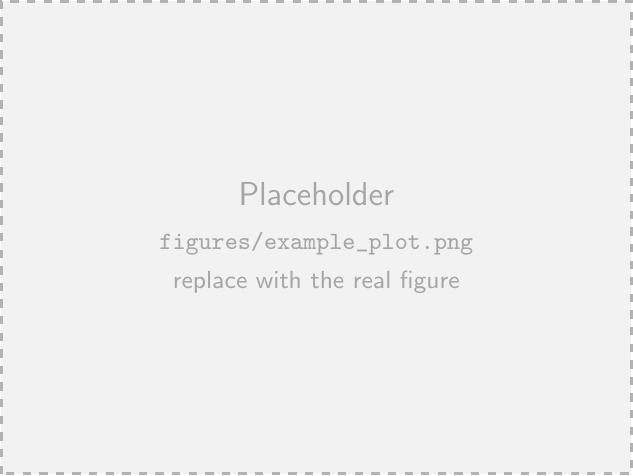
\includegraphics[width=\linewidth]{figures/example_plot.png}
    \caption{One-column figure that explains the steps or framework of your method / model.}
    \label{fig:one-col-figure}
\end{figure}

% figure* spans both columns; LaTeX places it at the top of a page.
\begin{figure*}
    \centering
    
\includegraphics[width=\linewidth]{figures/example_pipeline.png}
    \caption{One-column figure that explains the steps or framework of your method / model.}
    \label{fig:two-col-figure}
\end{figure*}

% ---------------------------------------------------------------------------
% 4. Experimental results  (TODO -- template text)
% ---------------------------------------------------------------------------
\section{Experimental Results}
\subsection{Datasets}
Include a description of the data used, what it contains, train test splits, etc.
\subsection{Implementation Details}
Include a description of the design choices, hyperparameters, and other implementation specific details.

\subsection{Results}
Analyze and discuss your results. Table \ref{tab:example-table} shows an example of a table.
Include plots and visualizations such as Figure \ref{fig:one-col-figure}.

\subsection{Discussion}
Additionally, you can include a separate discussion section in which you summarize the results, indicate possible limitations of your work, and provide suggestions for future research.

\subsection{Citing references}
LaTeX manages the citations for you. You simply have to add the bibtex entry for the reference in the references.bib file and you can use the citation in the paper \cite{langley00}. You can also cite multiple references in one command \cite{DudaHart2nd,Newell81,kearns89}. The bibtex entries for a paper can be obtained in websites such as google scholar or dblp.

% Note: \label must come after \caption, otherwise \ref points to the
% enclosing section instead of the table.
\begin{table}[h]
    \centering
    \caption{Example Table}
    \label{tab:example-table}
    \begin{tabular}{lllll}
        \toprule
        \multirow{2}{*}{Models} & \multicolumn{3}{c}{Metric 1} & Metric 2\\
        \cmidrule{2-4} \cmidrule{5-5} \\
        {} & precision & recall & F-score  & R@10 \\
        \midrule
        model 1 & 0.67  & 0.8 & 0.729  & 0.75 \\
        model 2 & 0.8 & 0.9 & 0.847 & 0.85 \\
        \bottomrule
    \end{tabular}
\end{table}

% ---------------------------------------------------------------------------
% References (entries live in references.bib)
% ---------------------------------------------------------------------------
\bibliography{references}
\bibliographystyle{icml2021}


\end{document}
